\documentclass[12pt]{article}
\usepackage[utf8]{inputenc}
\usepackage[greek,english]{babel}
\usepackage{alphabeta}
\usepackage{fancyhdr}
\usepackage{listings}
\usepackage{mathtools}
\usepackage{xcolor}
\usepackage{float}
\usepackage{siunitx}
\usepackage[margin=0.5in]{geometry}
\usepackage[backend=bibtex]{biblatex}

\lstset {
        basicstyle=\ttfamily,
        columns=fullflexible,
        breaklines=true,
        keepspaces=true,
	showstringspaces=false
}

\title{Εργαστήριο Προηγμένης Αρχιτεκτονικής Υπολογιστών -- Εργασία 1}
\author{Χρήστος Μαργιώλης -- 19390133}
\date{Μάρτιος 2025}

\begin{document}

\begin{titlepage}
        \maketitle
        \begin{figure}[t!]
        \begin{center}
        
\includegraphics[scale=0.3]{./res/uniwalogo.png} \\
        \Large
        \textbf{Πανεπιστήμιο Δυτικής Αττικής} \\
        \large
        Τμήμα Μηχανικών Πληροφορικής και Ηλεκτρονικών Υπολογιστών
        \end{center}
        \end{figure}
\end{titlepage}

\renewcommand{\contentsname}{Περιεχόμενα}
\tableofcontents
\pagebreak

\section{Προσαρμογή προσομοιωτή}

Απενεργοποίηση Enable Forwarding, Enable Target Buffer και Enable Delay Slot:
\\

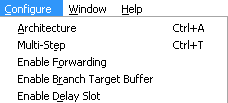
\includegraphics{res/disable.png} \\

Επαλήθευση τιμών παραμέτρων: FP Addition Latency = 4, Multiplier Latency = 7,
Division Latency = 24: \\

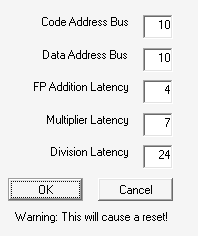
\includegraphics{res/latency.png}

\section{Ερώτημα 1}

\section{Ερώτημα 2}

Παρακάτω δίνονται οι χρόνοι εκτέλεσης (σε κύκλους ρολογιού) κάθε εντολής:

\begin{center}
\begin{tabular}{|l|l|}
	\hline
	\textbf{Εντολή} & \textbf{Κύκλοι} \\ 	
	\hline
	\lstinline|ddiv r18,r19,r20| & 28 \\
	\hline
	\lstinline|lw r1,4(r2)| & 5 \\
	\hline
	\lstinline|sw r3,8(r4)| & 5 \\
	\hline
	\lstinline|daddi r5,r6,10| & 5 \\
	\hline
	\lstinline|or r7,r8,r9| & 5 \\
	\hline
	\lstinline|dadd r10,r11,r0| & 5 \\
	\hline
	\lstinline|dsub r12,r13,r14| & 5 \\
	\hline
	\lstinline|dmul r15,r16,r17| & 11 \\
	\hline
	\lstinline|add.d f1,f2,f3| & 8 \\
	\hline
	\lstinline|mul.d f4,f5,f6| & 11 \\
	\hline
	\lstinline|halt| & 5 \\
	\hline
\end{tabular}
\end{center}

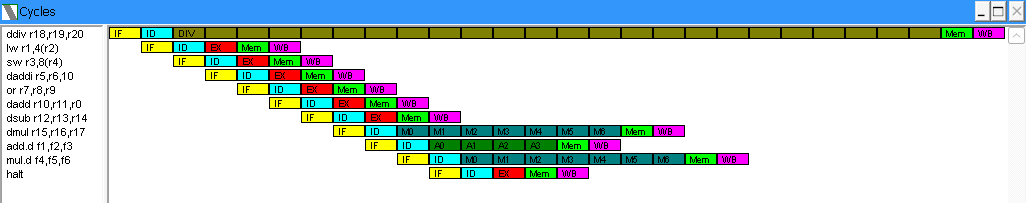
\includegraphics[width=\textwidth]{res/cycles.png}

\section{Ερώτημα 3}

Για την εκτέλεση όλου του κώδικα χρειάστηκαν 28 κύκλοι: \\

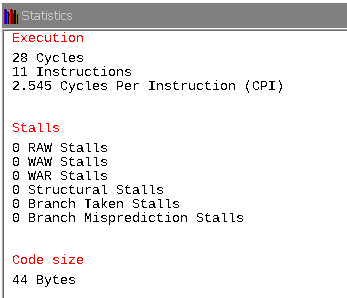
\includegraphics{res/total.png}

\section{Ερώτημα 4}

Το CPI (Cycles Per Instruction) είναι 2.545 (βλ. εικόνα ερωτήματος 3). Η τιμή του υπολογίζεται ως:

\[
	CPI = \frac{Cycles}{Instructions} = \frac{28}{11} \approx 2.545
\]

\end{document}
